%File: formatting-instruction.tex
\documentclass[letterpaper]{article}
\usepackage{aaai}
\usepackage{times}
\usepackage{helvet}
\usepackage{courier}
\usepackage{graphicx} 
\usepackage{caption}
\usepackage{gensymb}
\usepackage{hyperref}
\frenchspacing
\setlength{\pdfpagewidth}{8.5in}
\setlength{\pdfpageheight}{11in}
\pdfinfo{
/ (Sentence Writing Assistant Network: SWAN)
/Author (Jasper Eng and Firas Al Chalabi)}
\setcounter{secnumdepth}{0}  
 \begin{document}

% Sections:
%   Abstract
%   1. Motivation
%   2. Hardware
%   3. Design
%   4. software
%     4.1   Path planning / Letter design
%     4.2.  CV
%   5. Results
%   6. Future work 
%   7. Conclusion
 
\title{Sentence Writing Assistant Network: SWAN}
\author{Jasper Eng and Firas Al Chalabi}
\maketitle
\begin{abstract}
\begin{quote}
TODO
 This was done by designing a high precision robot that could take input as either text, or images of text. The end result was a robot that was able to write sentences within two line spaces on a standard sheet of paper.
\end{quote}
\end{abstract}

\section{1. Motivation}
The goal of this project was to design a system that allowed a user to interface with a robot that would be able to write clean legible sentences. The inspiration for this project was the fact that our own handwriting is quite bad, so we thought it would be interesting to see if we could create a system that was able to outperform our own writing. We also enjoyed the idea of creating highly precise (mm precision) robots with cheap and accessible resources.

\section{2. Hardware}
This section will provide a comprehensive list of parts that we used, and also how they were used in our design.
\subsection{2.1 Components}
We used: 3 Lego Ev3dev Large motors, two counterweights one weighing 3lbs and the other 5lbs, 1m of fishing line, 3 pieces of hardwood flooring, one two by four, one drawer pull unit, and lastly a sliding tray. In addition to these parts we used a few Lego pieces to supplement the build.\\\\
%
We used the motors as well as our counterweights and fishing line in order to get movement of our end effector in the x, y, and z direction. All of the wood in the build was used to design the frame on which the end effector was mounted. The sliding tray and drawer pulling unit were both used for fixing movement in one direction. Since both of these moved in fixed straight lines they were ideal for ensuring that when we rotated the motors we ended up with straight lines.  

\section{3. Design}
The design of our robot turned out to be critical to achieving the degree of accuracy that we needed. We went through many design ideas before deciding on our final build, this included and armed robot, a prismatic robot with a smaller robot mounted at the end effector for precision movement and finally our design of 2 prismatic joints. We took inspiration from 3D printer design, since they are also built for small precise movements.\\\\
%
In order to  turn the rotational motion of the motors into the linear motion we needed we spooled fishing line into coils above each of our motors. This of course would only allow the motor to pull an object towards itself, so in order to get movement in the opposite direction we used a counterweight attached to the other end of the string. This meant that when the motor unspooled the fishing line the counterweight would pull the object in the other direction. This design also came with the benefit that it was highly precise, allowing us to use the rather inaccurate Lego motors and still achieve millimeter precision. We believe the reason that the cables work so well is that they do not suffer from problems such as gear lashing.\\\\
% 
With the ability to use our motors for  linear motion we were able to create movement in the x, and y direction of our page. To do this we fixed our fishing line to objects that were fixed in their movement ie. our sliding tray, and drawer slider. The sliding tray was used to hold our paper, and served as our writing surface. While the drawer slider was used to mount our end effector, and the additional motor we used to get movement in the z direction. We then mounted the drawer slider to a wooden frame letting it sit over top of our writing surface. \\\\
%
The last step in our build process was to get z movement so we could lift our pen up from the page. To do this we fit the pen into a tube mounted to our drawer slider, then we inserted a pin into the top of our pen. Since the distance we needed to travel was quite small (< 3cm) we could simply attach a bar across the Lego motor and to the pin in the pen, then when the motor would rotate the pen would move up and down. With that completed we now had a robot that was accurate enough to perform the task outlined above, and we could begin work on designing the software. \\\\
%
The design outlined above is a description of our final build, each of the design aspects laid out went through many iterations of trial and error. Some more than others, for example one design aspect that caused us the most trouble was getting the pen to lift up -- the z motion. The fist iteration of this design relied on gears, but those proved to not be robust enough to even minor shifts in our environment. After many different design ideas we finally settled on the pin design highlighted above.

\section{4. Software}
There were 2 main software components in this project: path planning and computer vision.
\subsection{4.1 Path Planning}
\subsubsection{4.1.1 Drawing Simple Shapes\\}
To be able to draw any particular letter we needed to be able to draw the shapes that comprise that letter. We noticed that all uppercase letters in the English alphabet can be broken down into 4 main shapes: horizontal, vertical and diagonal lines, as well as quarter ellipses. Note that diagonal lines can face forwards or backwards, and that quarter ellipses can have any orientation based on the 4 quadrants of a Cartesian plane (see Figure 4.1 below). 

\begin{figure}[http]
    \centering
    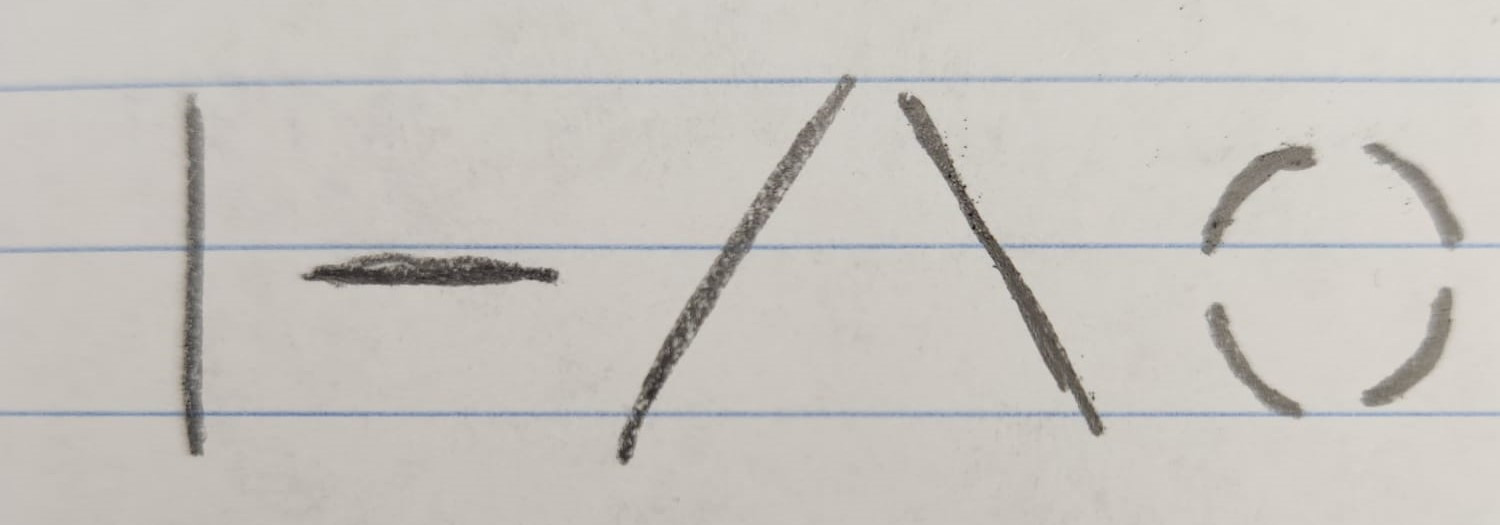
\includegraphics[width=4cm]{Simple Shapes.jpg}
    \caption*{Figure 4.1. The simple shapes that comprise all uppercase letters.}
    \label{fig 4.1}
\end{figure}
The way we draw horizontal lines is by moving the servo motor attached to the drawer pulling unit (subsequently referred to as the x-motor), and vertical lines by moving the servo motor attached to the sliding tray (subsequently referred to as the y-motor). Assume that if we want to draw a straight line that is $1$ unit long in a specific direction we rotate the corresponding motor by $\theta\degree$. The direction of rotation determined the path that would be taken when drawing a particular shape. We drew diagonal lines by moving both motors at the same time, and we made sure that both motors stopped at the same time by adjusting the ratio of their speeds according to how long we wanted the diagonal line to be in both the x-direction and the y-direction. For example, if we wanted a diagonal line that extended $0.5$ units in the x-direction and $2$ units in the y-direction, we would have the x-motor $0.5\theta\degree$ and the y-motor $2\theta\degree$ while simultaneously moving the x-motor at a quarter of the y-motor's speed (as $0.5/2 = 1/4$). As for quarter ellipses, we broke them down into a series of diagonal lines with different lengths in the x- and y-directions. We calculated those lengths programmatically using the sine and cosine functions. 
%
\subsubsection{4.1.2 Drawing Letters\\}
Once we were able to draw the simple shapes that comprise the uppercase letters (see above), the next step was to break down each letter into those shapes (see Figure 4.2). We decided that each letter was to be bounded in a box that was $2$ units long and $1$ unit wide (see Figure 4.3), and that we can assume that the pen will always start at the bottom left corner of said box. This way, we can draw each letter without having to factor in our current position on the paper, or account for the previous letter drawn.
\begin{figure}[http]
    \centering
    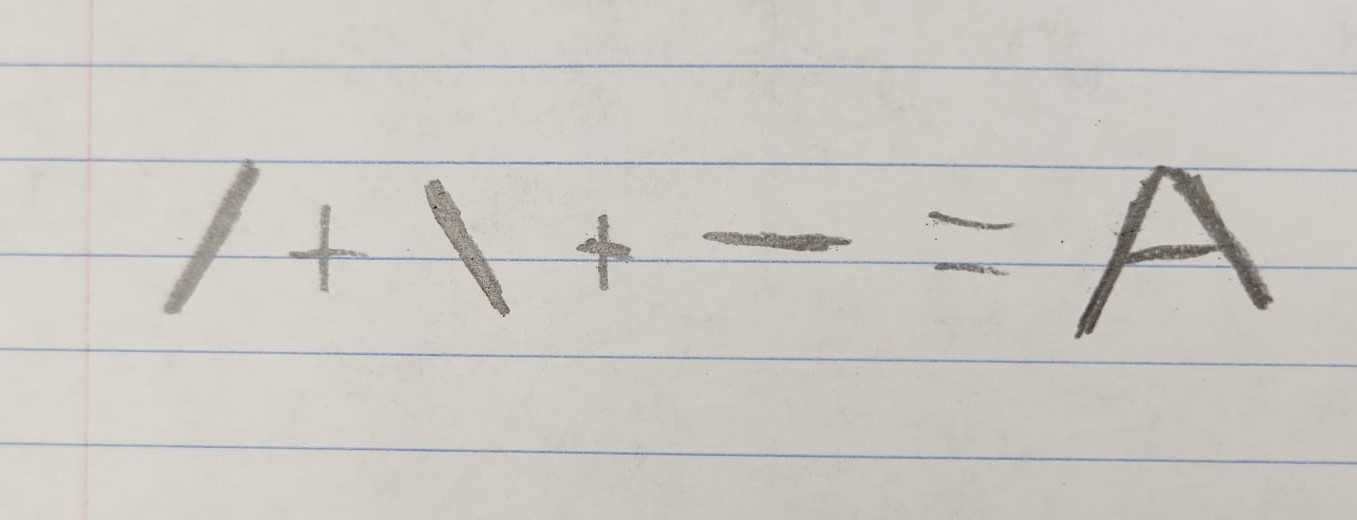
\includegraphics[width=0.5\linewidth]{A components.jpg}
    \caption*{Breaking down the letter A into its components.}
    \label{fig:4.2}
\end{figure}
\begin{figure}[http]
    \centering
    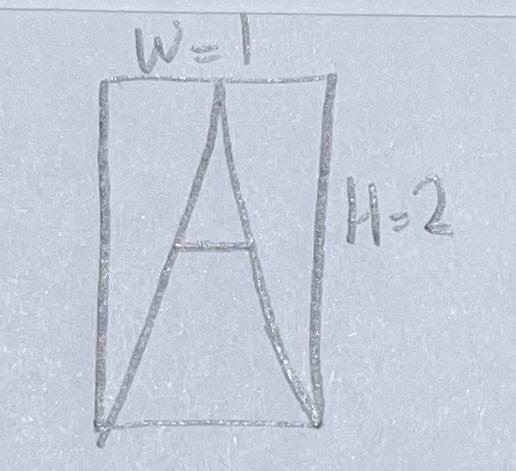
\includegraphics[width=0.5\linewidth]{A - Bounding Box.jpg}
    \caption*{An example of the letter A in its bounding box.}
    \label{fig:4.3}
\end{figure}
\subsubsection{4.1.3 Writing Words and Sentences}
The way we designed our letter-drawing workflow made it relatively easy to write complete words. Since, for each letter, the pen would start and end on the bottom left corner of the bounding box (in the pen-up position), moving on to the next letter was simply a matter of moving in the x-direction by $1.25$ units. We determined that $0.25$ units was an appropriate spacing between a letter and the next by testing different values. To get spaces between words, we just "skip" a letter, i.e. we lift the pen up and move the motor the width of one letter from where the next letter was supposed to start. We keep track of the number of letters we have drawn per line, and when we're about to exceed that amount, or we encounter a newline character, we move our pen down (in the y-direction) 2.25 units, and we move back the width of the number of letters including the spaces between letters.
%
\subsubsection{4.1.4 Implementing Different Font Sizes}
We wanted our robot to write words and sentences in different font sizes. We started by defining our maximum font size, which maps $1$ unit in either the x- or y-directions to $1$ full rotation of the corresponding motor. The width of our workspace was 32 cm (width)

\subsection{4.2 Detecting Letters From Images}
Once we were able to draw letters we also wanted to create multiple different interfaces for the user to interact with our robot. The easiest way is to just have the user enter text into a terminal and pass the string to the robot for writing. However we also wanted for the robot to be able to recreate sentences written by a human, to do this we designed a system where the user pass an image to the robot and it would convert the image to a string that could be passed to the robot.
\subsubsection{4.2.1 Pre-Processing}
The first step in this process was to get characters from an image. To do this we would read the image in grey scale, and then perform a colour thresholding operation in order to identify all parts of the image that were letters. Once we had done that we could draw bounding boxes around each of the regions of interest. The issue with doing this on the original image was that humans do not write each letter evenly spaced, meaning that the bounding box for one letter would often contain parts of another letter, see fig 4.3. \\
\begin{figure}[http]
    \centering
    
\includegraphics[width=3cm]{Overlap.jpg}
    \caption*{Figure 4.3. This image shows how parts of other letters can be present in the bounding boxes of different letters. In the upper left corner there is an artifact from a different letter in the bounding box of the "a".}
    \label{fig 4.3}
\end{figure}\\
To solve this problem we projected the letter who's ROI we were looking at onto a blank black image. This removed any extra noise in the image, and only left the outlined letter. The last step in the pre-processing step was to make sure we had the correct ordering of letters. To do this we just put the bounded images into a list sorted by the x coordinate of their upper left corner. Meaning that we now had a list of images that went from the leftmost letter to rightmost. \\\\
%
We can now take this list and pass each image into a classification model in order to determine which letter we are looking at. Before doing that we make sure that all images are the correct size, and format for our model to accept.
\subsubsection{4.2.2 Classification}
The next step in our computer vision pipeline is to classify an image of a letter. To do this we tried two different classification architectures, a Visual Transformer, and a Convolutional Neural Network. The structure of the ViT 

\end{document}